\chapter{Model Configuration Management in MADTrack}\label{cap:Milestone2}

This chapter covers the development of milestone 2 (codename \emph{M}), related to the development of features related to configuration
management applied to \acrshort{AI} models. This module will provide great value to the end user, increasing the reproducibility of the
trainings performed on a given model. For this reasons, this is the chapter with the most prototypes to be developed, and the one with 
the most complex architecture.

\section{Introduction}

This chapter aims to provide the necessary documentation of the development of the requirements and features necessary for the fulfillment
of one of the partial objectives of the project, which consists in developing a module for versioning \acrshort{AI} models. This module will
integrate a vital component for deployment, the MADTrack Tracking Server, which will handle the requests from users and store the training 
configurations. This component, along with the developed solution for the target system that will be used to register the traings, will ensure
every single training is accessible for the users, and can be reproduced with similar results in the future.

\section{Requirements analysis for milestone 2}

Just as with the other milestones, an analysis of the requirements will be performed to define a high-level outline of what is to come on the 
following sections. First, the requirements will be grouped semantically according to the milestone 1 prototype that suits best for each requirement,
and then make a study of what application type and architecture is more suitable for the module, and what toolkits out of the ones explored on 
\emph{Chapter \ref{cap:StateOfTheArt}} would be the most helpful to develop the prototype.

\subsection{Requirements involved}

Just like milestone 1, milestone 2 has a set of requirements that have to be semantically divided into the different prototypes. The requirements belonging
to milestone 2 (those with the prefix \emph{MFR}) have been already listed within \emph{table \ref{tab:functionalRequirements}}, and now they will be divided
into three prototypes: \emph{M1} (requirement listed within \emph{table \ref{tab:requirementsM1}}), \emph{M2} (requirement listed within \emph{table \ref{tab:requirementsM2}}),
and \emph{M3} (requirement listed within \emph{table \ref{tab:requirementsM3}}).

\begin{table}[H]
    \centering
    \begin{tabular}{ | c | p{9cm} | p{3cm} |}
        \hline
        \textbf{Requirement ID} & \textbf{Requirement Description} & \textbf{priority (MoSCoW)} \\ \hline
        MFR1     & The system MUST handle the concept of experiments. & Must have \\ \hline
        MFR1.1   & The system MUST identify an experiment by its identification string, or ID. & Must have \\ \hline
        MFR1.2   & The system MUST provide a mechanism for creating experiments. & Must have \\ \hline
        MFR1.3   & The system MUST not accept an experiment creation request that has no experiment name. & Must have \\ \hline
        MFR1.4   & The system MUST separate commits from different experiments. & Must have \\ \hline
        MFR1.5   & The system MUST provide a mechanism for deleting experiments. & Must have \\ \hline
        MFR1.6   & The system MUST provide a mechanism for switching between experiments. & Must have \\ \hline
    \end{tabular}
    \caption{Requirements for prototype \emph{M1}.}
    \label{tab:requirementsM1}
\end{table}

\begin{table}[H]
    \centering
    \begin{tabular}{ | c | p{9cm} | p{3cm} |}
        \hline
        \textbf{Requirement ID} & \textbf{Requirement Description} & \textbf{priority (MoSCoW)} \\ \hline
        MFR2     & The system MUST keep ordered track of machine learning model configurations. & Must have \\ \hline
        MFR2.1   & The system MUST track which dataset was used to train the model. & Must have \\ \hline
        MFR2.2   & The system MUST track which dataset was used to validate the model. & Must have \\ \hline
        MFR2.3   & The system MUST track which dataset was used to test the model. & Must have \\ \hline
        MFR2.4   & The system MUST track the code used for programming the model's training. & Must have \\ \hline
        MFR2.5   & The system MUST track the configuration of the model's hyperparameters and random parameters used in the training of an AI model. & Must have \\ \hline
        MFR2.6   & The system MUST track the metrics achieved by an AI model. & Must have \\ \hline
        MFR2.7   & The system MUST provide users with a mechanism to mark an AI model as currently deployed. & Should have \\ \hline
        MFR2.8   & The system MUST keep track of the additional parameters used by an AI model if it handles domain-specific data. This will be tested for the domain of Earth Observation. & Must have \\ \hline
    \end{tabular}
    \caption{Requirements for prototype \emph{M2}.}
    \label{tab:requirementsM2}
\end{table}

\begin{table}[H]
    \centering
    \begin{tabular}{ | c | p{9cm} | p{3cm} |}
        \hline
        \textbf{Requirement ID} & \textbf{Requirement Description} & \textbf{priority (MoSCoW)} \\ \hline
        MFR3     & The system MUST provide a mechanism for evaluating an AI model's metrics' goodness. & Should have \\ \hline
        MFR3.1   & The system MUST provide a mechanism for choosing policies to evaluate an AI model's metrics' goodness. & Should have \\ \hline
        MFR3.2   & The system MUST provide a mechanism for identifying the experiment or model with the best values on the chosen metrics. & Should have \\ \hline
        MFR3.3   & The system SHOULD order the model trainings made on an experiment by the goodness of the values on the chosen metrics. & Should have \\ \hline
        MFR4     & The system MUST provide a mechanism for visualizing the performance report for a trained AI model (if any). & Should have \\ \hline
        MFR5     & The system MUST provide a mechanism to visualize the training graph of a model (this is, the graph that describes the progress of the metrics of a model after each epoch). & Could have \\ \hline
    \end{tabular}
    \caption{Requirements for prototype \emph{M3}.}
    \label{tab:requirementsM3}
\end{table}

\subsection{Integration with the rest of the system}

Prototypes within milestone 2 have a strong relation with the rest of milestones, since they need the configuration management mechanisms to commit changes made to the folders that track
the model training configurations, and will also use the dataset versioning system on dataset logging tasks.

\begin{figure}[H]
    \centering
    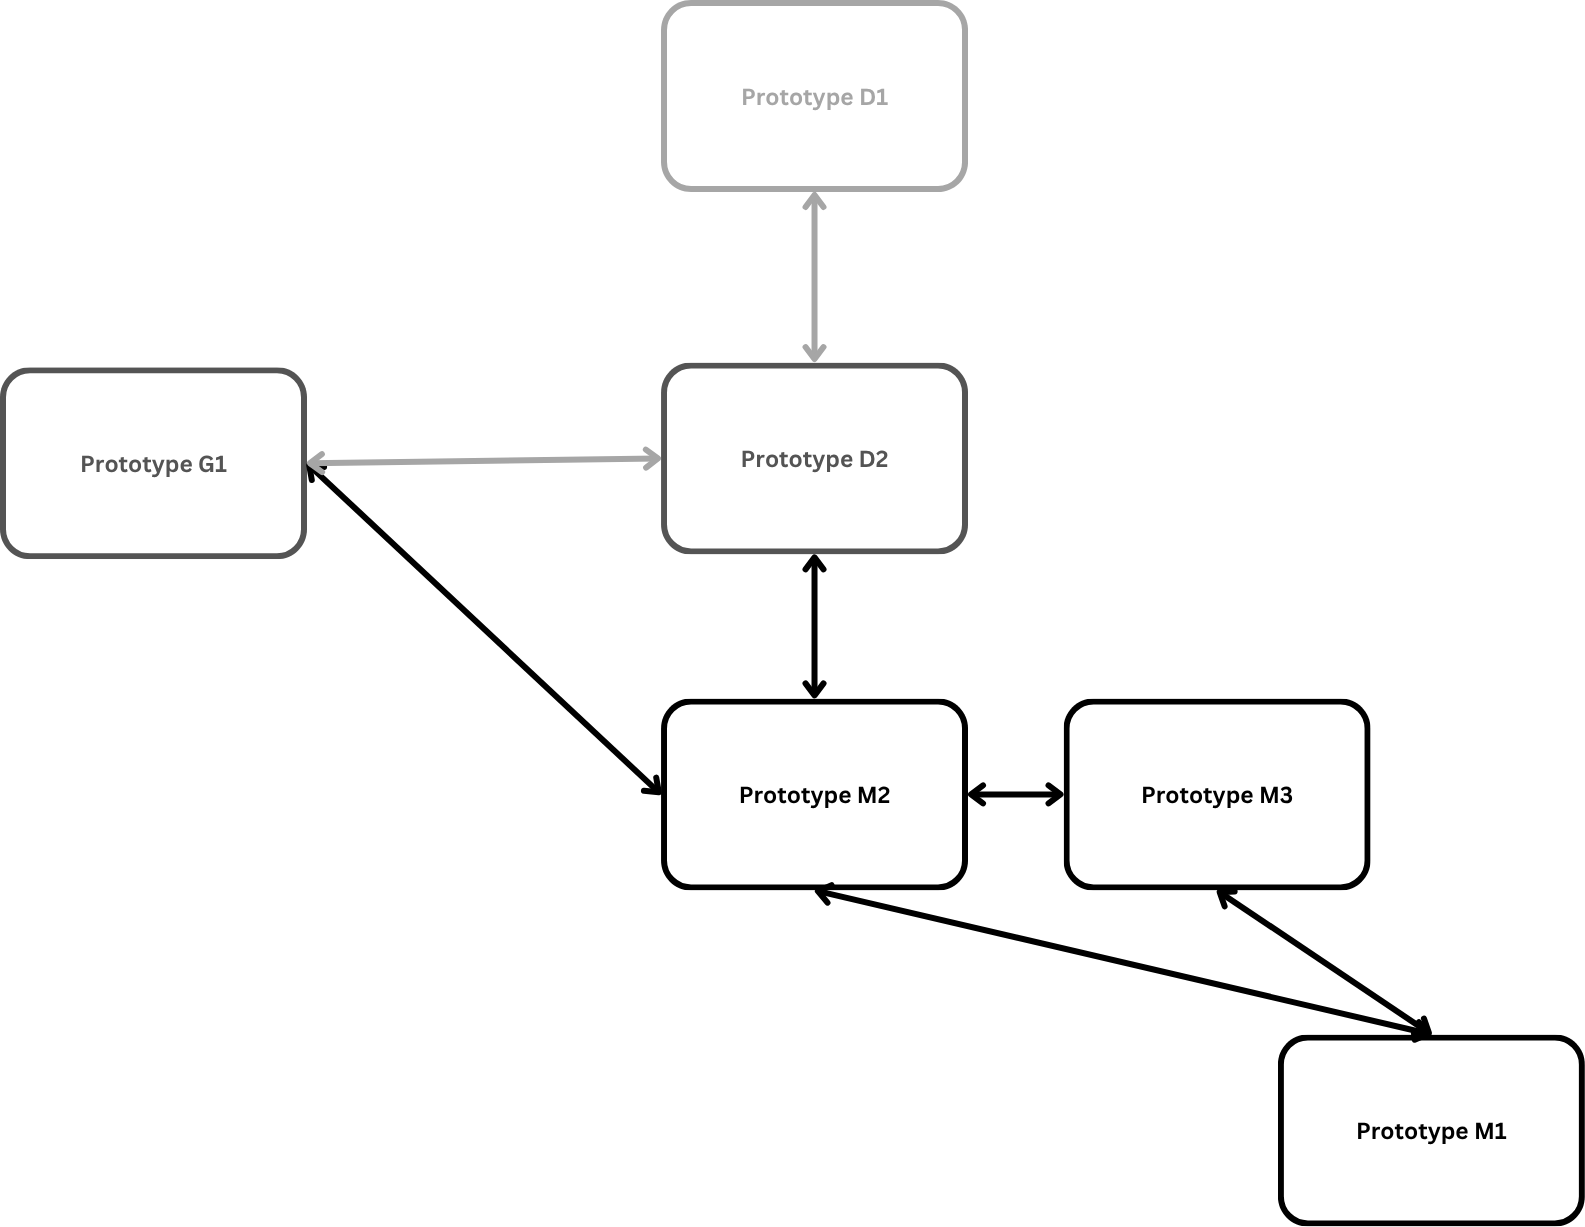
\includegraphics[width=0.7\textwidth]{figs/M-dependencies.png}
    \caption{Dependencies between prototypes of milestone 2 and the rest of the target system, shown by an interaction diagram.}
\end{figure}

\subsection{Architecture analysis}

The main objective of the milestone is to enable the target system to handle experiments, model trainings, register and version them. The need for
registration of events happening on a machine at the time they are happening arise the need of a component that can manage all of them. This component
shall be separate from the rest of the system so as to increase portability. Hence, the architecture of this module will be distributed, with two main components.

\subsection{Application type analysis}

The aim of this prototype is to manage the existence of experiments. Since this is a double-sided task, the best approach is to provide the 
management functionality inside a Wrapper Library, from which the user will be able to create, delete and switch their active experiment, as well
as managing their model trainings using code, whilst a remote tracking server will be in charge of processing these requests with a web 
application, provided by an external toolkit.

\subsection{Toolkit analysis}

The most suitable toolkit for the development of this milestone is the one that provides a mechanism for creating experiments under the 
definition of a series of \acrshort{AI} model lifecycles performed with the purpose to achieve a suitable model for a specific goal. A nice example is MLFlow
(overviewed in \emph{Chapter \ref{cap:StateOfTheArt}}), which is a tool for model registration and experiment tracking.

\section{Prototype design and development}

The following subsections contain details about the design, implementation and teting process for the three prototypes this milestone is composed of.

\subsection{Prototype \emph{M1}}

Prototype \emph{M1} is the first stage of development of Milestone 2 (consisting in \acrshort{AI} model versioning and tracking). The objective of this prototype is to provide 
the necessary mechanisms to register experiments into a remote server, based on their purpose.

\subsubsection{Design for prototype \emph{M1}}

The following sections describe the design process of prototype \emph{M1}.

\paragraph{Components for prototype \emph{M1}} \mbox{}\\

The use case diagram which summarizes this prototype's needs is shown in \emph{figure \ref{fig:useCaseM1}}.

\begin{figure}[H]
    \centering
    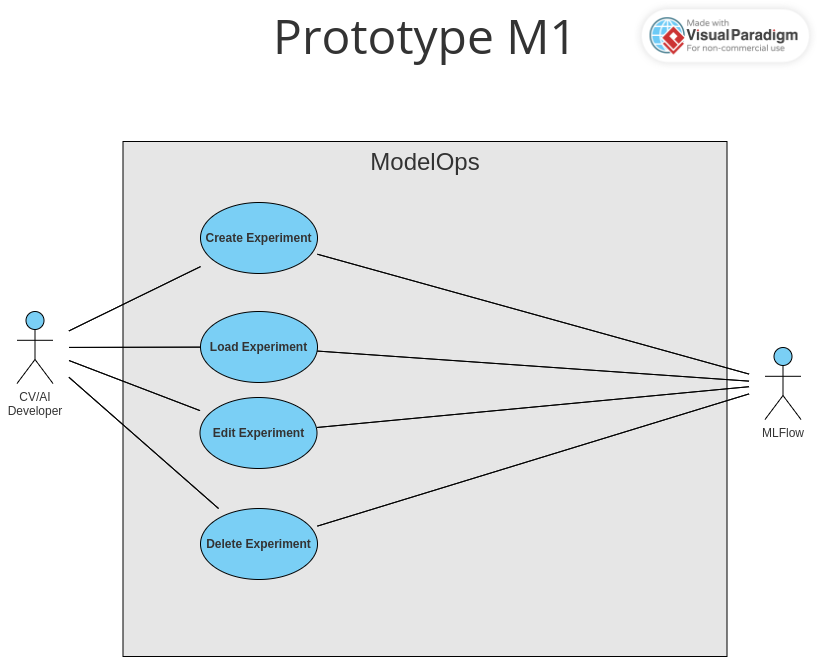
\includegraphics[width=0.7\linewidth]{figs/use-case-M1.png}
    \caption{Use case diagram for prototype \emph{M1}.}
    \label{fig:useCaseM1}
\end{figure}

The objective of this prototype is to handle the life cycle of experiments: creation, switching,
edition and deletion. For this purpose, a new class with the role of managing this life cycle will be created, along with a new component which 
will relate to deployment:

\begin{itemize}
    \item \textbf{Experiment Manager: }this class will yield the role of managing the life cycle of experiments, covering all the aforementioned 
    operations. It will be able to create, switch, edit and delete experiments.

    \item \textbf{Tracking Server: }a Distributed component consisting on a docker container, running locally for the meantime, which will contain
    the Active MADTrack Tracking server which will use a file system as storage.

    \item \textbf{Model Tracking Exceptions }: a package that includes some special exceptions that can be raised by the Experiment Manager. 
\end{itemize}

\paragraph{Design output for prototype \emph{M1}}\mbox{}\\

The design class diagram for prototype \emph{M1} is shown in \emph{Placeholder for annex figure}.

\subsubsection{Implementation for prototype \emph{M1}}

The following lines describe the details of the implementation of the prototype.

\paragraph{Libraries} \mbox{}\\

The libraries used for this implementation are:

\begin{itemize}
    \item \textbf{MLFlow: }an open-source Python library that provides a unified API for tracking and logging machine learning experiments.
    \item \textbf{Logging: }a library that enables the creation of log files and manages log operations within any Python application.
    \item \textbf{OS: }a Python library enabling operating system interaction. It will be used to build the necessary paths to local file repositories.
    \item \textbf{YAML: }A Python library that provides a way to represent data in YAML format using simple structures.
\end{itemize}

\subsubsection{Testing for prototype \emph{M1}}

The following paragraphs contain information about the test suites and errors fixed during the testing process of prototype \emph{M1}.

\paragraph{Test suites for Experiment Manager}\mbox{}\\

The test suites for this prototypes can be found in \emph{annex reference placeholder}. % Referencia al Anexo con las tablas (porque pueden ser muy grandes y no es plan). Esto no es prioritario, puede esperar

\paragraph{Errors found and lessons learned during the development of prototype \emph{M1}}\mbox{}\\

The errors encountered during the course of the testing phase of prototype \emph{M1} are shown in \emph{annex reference placeholder}. % De nuevo, esto puede esperar porque va al anexo

\subsection{Prototype \emph{M2}}

Prototype \emph{M2} is the second stage of development of milestone 2. This prototype will focus on the 
effective \acrshort{AI} logging during the model lifecycle. This objective can be accomplished by providing mechanisms for logging all 
the datasets (test, train, validation), the code used to train the model, the hyperparameters, and domain-specific data.

\subsubsection{Design for prototype \emph{M2}}

The following sections describe the design process of prototype \emph{M2}.

\paragraph{Components for prototype \emph{M2}} \mbox{}\\

First, it is necessary to look at the use case diagram, (shown at \emph{figure \ref{fig:useCaseM2}}), which summarizes this prototype's needs.

\begin{figure}[H]
    \centering
    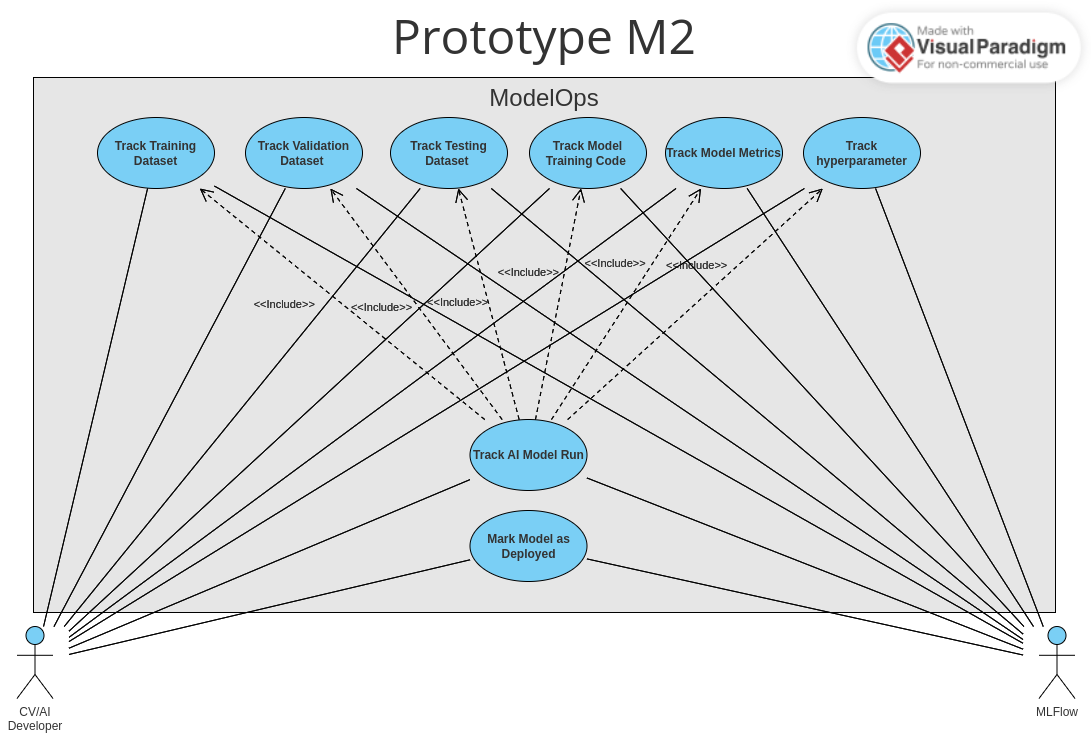
\includegraphics[width=0.7\linewidth]{figs/use-case-M2.png}
    \caption{Use case diagram for prototype \emph{M2}.}
    \label{fig:useCaseM2}
\end{figure}

The objective of this prototype is to enable users to fill their experiments with \emph{Model Runs} (for more information about these, please refer to
\emph{section \ref{sec:mlflow}}), which will have several data logged according to the needs of the user. For this objective, a new component will be created 
to represent an \acrshort{AI} model run, along with changes in the Experiment Manager component. The list of components involved in this prototype is:

\begin{itemize}
    \item \textbf{Model Run:} This component will be in charge of representing a run of a single model within the training workflow. Its main functionality
    resides in the component's capability of logging the necessary items to store the configuration of a run.

    \item \textbf{Experiment Manager: }This class will enjoy new functionalities, such as the capability to run a complete run workflow or to register a new \acrshort{AI} 
    model version within the model registry.

    \item \textbf{Tracking Server: }This component will be able to store the necessary data to enable logging in the model run. The details about its architecture are revealed in \emph{Chapter }
\end{itemize}

\paragraph{Design output for prototype \emph{M2}}\mbox{}\\

The design class diagram for prototype M2 is shown in \emph{Placeholder for annex figure}.

\subsubsection{Implementation for prototype \emph{M2}}

This are the lines that contain the main details about this prototypes implementation. The main libraries do not differ from
the previous prototype.

\subsubsection{Testing for prototype \emph{M2}}

The particularity of the testing of this prototype is that it could be mostly done from the Experiment Manager component, since it has a method that subcalls the methods
from the Model Run component. The test suites of the Experiment Manager will also test the Model Run component.

\paragraph{Test suites for prototype \emph{M2}}\mbox{}\\

The test suites for this class can be found in \emph{annex reference placeholder}.

\paragraph{Errors found and lessons learned}\mbox{}\\

The errors encountered during the course of the testing phase of prototype \emph{M2} are shown in \emph{annex reference placeholder}.

\subsection{Prototype \emph{M3}}

Prototype M3 is the third stage of development of Milestone M (AI model versioning and tracking). This prototype will be focused on how metrics are shown in the
MADTrack system and how they are presented to end users, as well as the final presentation of these metrics on a performance report (Which would be logged as 
another parameter and printed out when completing a Model Run, if necessary).

\subsubsection{Design for prototype \emph{M3}}

The following sections describe the design process of prototype \emph{M3}.

\paragraph{Components for prototype \emph{M3}} \mbox{}\\

The use case diagram is shown in \emph{figure \ref{fig:useCaseM3}}, summarizing thus the needs of this prototype.

\begin{figure}[H]
    \centering
    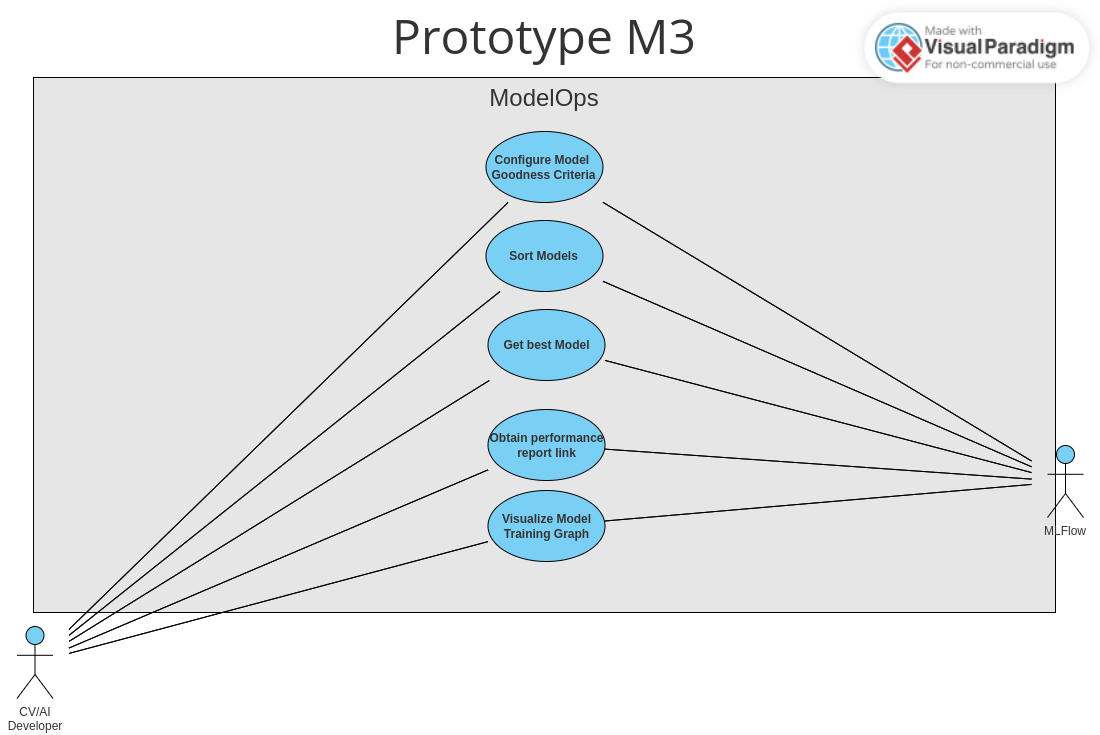
\includegraphics[width=0.7\linewidth]{figs/use-case-M3.png}
    \caption{Use case diagram for prototype \emph{M3}.}
    \label{fig:useCaseM3}
\end{figure}

The objective of this prototype is to enable users to extend the functionality of a model run, so that the goodness of the metrics can be configurable, so that the 
model runs can be sorted according to a specific metric, and so that the best model run can be highlighted in some way. Additionally, the system will also provide a 
mechanism to log a performance report for the model, which will be stored as an artifact of the model run and its access will also be provided in the logs, and to 
visualize the training graph of the model, if it is trained.

For this reason, the main component involved within this prototype is the Model Run component, which will gain additional methods, and the Experiment Manager component.

\paragraph{Design output for prototype \emph{M3}}\mbox{}\\

The design class diagram for prototype M3 is shown in \emph{Placeholder for annex figure}.

\subsubsection{Implementation for prototype \emph{M3}}

The following sections describe the implementation process of prototype \emph{M3}. The language and the libraries used are the same as the rest of prototypes of this milestone.

\subsubsection{Testing for prototype \emph{M3}}

The main testing methods focus on the new methods of the Model Run component.

\paragraph{Test suites for prototype \emph{M3}}\mbox{}\\

The test suites for this class can be found in \emph{annex reference placeholder}.

\paragraph{Errors found and lessons learned during the development of prototype \emph{M3}}\mbox{}\\

The errors encountered during the course of the testing phase of prototype \emph{M3} are shown in \emph{annex reference placeholder}.
